\documentclass[12pt]{exam}

\usepackage[brazil]{babel}   
\usepackage[TS1,T1]{fontenc}
\usepackage[utf8]{luainputenc}
\usepackage[utf8]{inputenc}  
%\usepackage[T1]{fontenc}
\usepackage{amsfonts,amsmath,amssymb,latexsym} 
\usepackage{enumerate}
\usepackage{float}
\usepackage{graphicx}
\usepackage{caption}
\usepackage{subcaption}
\graphicspath{ {images/} }




\def\cQ{\mathcal{Q}}
\def\ve{\varepsilon}

\def\emptyset{\varnothing}
\def\ept{\varnothing}

% Include the listings-package
\usepackage{listings}             
\usepackage{color}

\definecolor{dkgreen}{rgb}{0,0.6,0}
\definecolor{gray}{rgb}{0.5,0.5,0.5}
\definecolor{mauve}{rgb}{0.58,0,0.82}

\lstset{frame=tb,
  language=Prolog,
  aboveskip=3mm,
  belowskip=3mm,
  showstringspaces=false,
  columns=flexible,
  basicstyle={\small\ttfamily},
  numbers=left,
  stepnumber=1,  
  numberstyle=\tiny\color{gray},
  keywordstyle=\color{blue},
  commentstyle=\color{dkgreen},
  stringstyle=\color{mauve},
  breaklines=true,
  breakatwhitespace=true,
  tabsize=3
}


\usepackage{tikz}
\usetikzlibrary{trees}



\usepackage[margin=1in]{geometry}
\usepackage{amsmath,amssymb}
\usepackage{multicol}

\def\code#1{\texttt{#1}}

\newcommand{\class}{Computação Gráfica}
\newcommand{\term}{1º semestre de 2021}
\newcommand{\examnum}{Lista 01}
\newcommand{\examdate}{}

\pointpoints{ponto}{pontos}

\pagestyle{head}
\firstpageheader{}{}{}
\runningheader{\class}{\examnum\ - Página \thepage\ de \numpages}{\examdate}
\runningheadrule


\begin{document}

\noindent
\begin{tabular*}{\textwidth}{l @{\extracolsep{\fill}} r @{\extracolsep{6pt}} l}
\textbf{\class} & \textbf{Nome:} & \makebox[2in]{\hrulefill}\\
\textbf{\term}  & \textbf{RA:}   & \makebox[2in]{\hrulefill}\\
\textbf{\examnum} &&\\
& Professor: & Vinicius Pereira
\end{tabular*}\\
\rule[2ex]{\textwidth}{2pt}

Esta lista contém \numpages\ páginas e \numquestions\ questões.\\


\noindent
\rule[2ex]{\textwidth}{2pt}



\begin{questions}

\question Escreva a equação cartesiana e a equação paramétrica que representem a elípse abaixo. Considere que a elipse está com o ponto central em $(0, 0)$ e tem largura $2a$ e altura $2b$.

\begin{figure}[h]
    \centering
    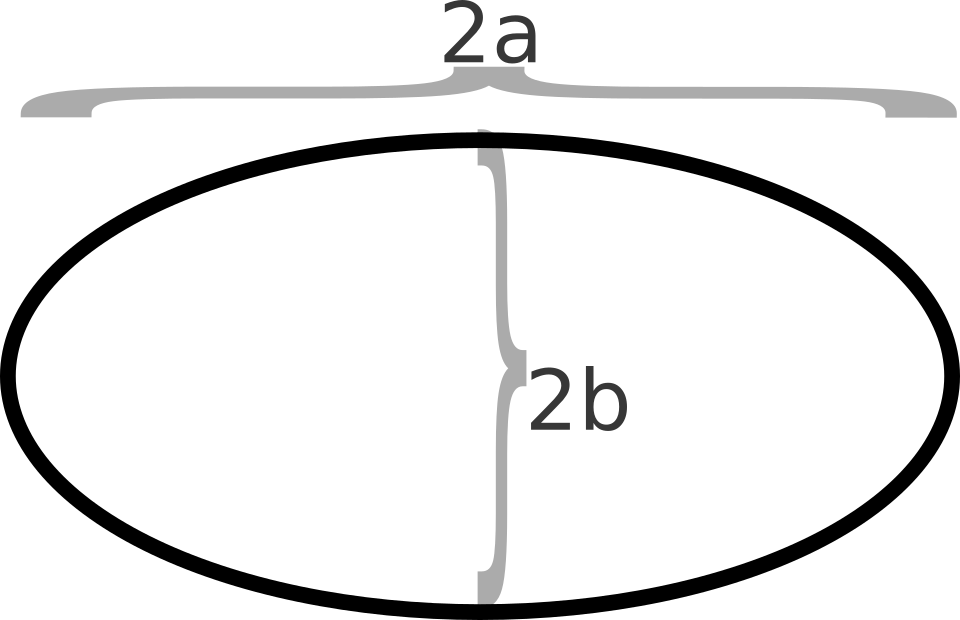
\includegraphics[width=0.5\textwidth]{elipse}
    \caption{Elipse}
    \label{fig:elipse}
\end{figure}

\question Desenhe o as seguintes curvas:

\begin{enumerate}[a)]

\item A curva definida pela seguinte equação cartesiana: $y = x$

\item A curva definida pela seguinte equação paramétrica: 
\[\begin{cases}
    x=t\\
    y=t
\end{cases}
t\in (-\infty,\infty)\]

\item A curva definida pela seguinte equação cartesiana: $y = 2x$

\item A curva definida pela seguinte equação paramétrica: 
\[\begin{cases}
    x=t\\
    y=2t
\end{cases}
t\in (-\infty,\infty)\]

\item A curva definida pela seguinte equação cartesiana: $y = x + 2$

\item A curva definida pela seguinte equação paramétrica: 
\[\begin{cases}
    x=t\\
    y=t + 2
\end{cases}
t\in (-\infty,\infty)\]

\item A curva definida pela seguinte equação cartesiana: $y = x^2$

\item A curva definida pela seguinte equação paramétrica: 
\[\begin{cases}
    x=t\\
    y=t^2
\end{cases}
t\in (-\infty,\infty)\]

\item A curva definida pela seguinte equação cartesiana: $1 = x^2 + y^2$

\item A curva definida pela seguinte equação paramétrica: 
\[\begin{cases}
    x=\cos (t)\\
    y=\sin (t)
\end{cases}
t\in (0, 2\pi)\]

\item A curva definida pela seguinte equação cartesiana: $4 = x^2 + y^2$

\item A curva definida pela seguinte equação paramétrica: 
\[\begin{cases}
    x=2\cos (t)\\
    y=2\sin (t)
\end{cases}
t\in (0, 2\pi)\]

\end{enumerate}

\break

\question Reescreva as seguintes curvas:

\begin{itemize}

\item após uma translação de 2 unidades na direção de $x$

\item após uma transformação de rotação de $90^\circ$

\item após uma transformação de escala de $2$ em ambos

\item após uma transformação de escala de $2$ no eixo $y$

\item após uma transformação de escala de $2$ no eixo $x$

\end{itemize}

reescreva para cada transformação separada.

\begin{enumerate}[a)]

\item A curva definida pela seguinte equação cartesiana: $y = x$

\item A curva definida pela seguinte equação paramétrica: 
\[\begin{cases}
    x=t\\
    y=t
\end{cases}
t\in (-\infty,\infty)\]

\item A curva definida pela seguinte equação cartesiana: $y = 2x$

\item A curva definida pela seguinte equação paramétrica: 
\[\begin{cases}
    x=t\\
    y=2t
\end{cases}
t\in (-\infty,\infty)\]

\item A curva definida pela seguinte equação cartesiana: $y = x^2$

\item A curva definida pela seguinte equação paramétrica: 
\[\begin{cases}
    x=t\\
    y=t^2
\end{cases}
t\in (-\infty,\infty)\]

\item A curva definida pela seguinte equação cartesiana: $1 = x^2 + y^2$

\item A curva definida pela seguinte equação paramétrica: 
\[\begin{cases}
    x=\cos (t)\\
    y=\sin (t)
\end{cases}
t\in (0, 2\pi)\]


\end{enumerate}



\break

\question Calcule as matrizes seguintes:

\begin{itemize}

\item A matriz responsável por fazer uma rotação de 90º, e em seguida uma escala de $2$ nos dois eixos.

\item A matriz responsável por fazer uma escala de $2$ nos dois eixos, e em seguida uma rotação de 90º.

\item As duas matrizes resultantes são iguais? Podemos concluir que a ordem das transformações não altera o resultado?

\end{itemize}

\question Calcule as matrizes seguintes:

\begin{itemize}

\item A matriz responsável por fazer uma rotação de $90^\circ$, e em seguida uma escala de $2$ \textbf{apenas} no eixo $x$.

\item A matriz responsável por fazer uma escala de $2$ \textbf{apenas} no eixo $x$, e em seguida uma rotação de $90^\circ$.

\item As duas matrizes resultantes são iguais? Podemos concluir que a ordem das transformações não altera o resultado?

\end{itemize}

\question Calcule as matrizes seguintes nas \textbf{coordenadas homogêneas}:

\begin{itemize}

\item A matriz responsável por fazer uma rotação de $90^\circ$, e em seguida uma translação de $2$ unidades em direção ao eixo $x$.

\item A matriz responsável por fazer uma translação de $2$ unidades em direção ao eixo $x$, e em seguida uma rotação de $90^\circ$.

\item As duas matrizes resultantes são iguais? Podemos concluir que a ordem das transformações não altera o resultado?

\end{itemize}


\end{questions}

\end{document}

